\chapter{Potenza lungo una Linea senza Perdite}
\section{Linea indefinita}
\begin{center}
    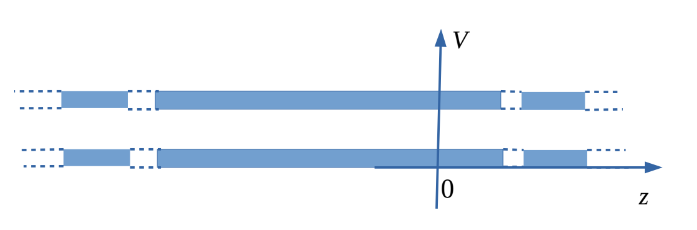
\includegraphics[width=0.8\textwidth]{Images/Figure13.png}
\end{center}
Lungo questa \textbf{linea senza perdite} si propaga la sola onda:
\begin{equation*}
    \begin{dcases}
    V(z) = V^+ e^{-jkz}\\
    I(z) = \frac{V^+}{Z_0} e^{-jkz}
    \end{dcases}
\end{equation*}
Valutiamo ora la potenza su un'ascissa generica:
\begin{equation*}
    P(z) = \frac{1}{2} V(z) I^*(z) = \frac{1}{2} V^+ e^{-jkz} \frac{{V^+}^*}{Z_0}e^{jkz} =  \frac{1}{2} \frac{|V^+|^2}{Z_0}
\end{equation*}
\section{Due Linee Indefinite}
Consideriamo ora il seguente schema:
\begin{center}
    \includegraphics[width=0.8\textwidth]{Images/Figure14.png}
\end{center}
\begin{equation*}
\tag{Prima Linea}
\begin{dcases}
    V_0(z) = V_0^+ e^{-jk_0z} +  V_0^- e^{jk_0z} = V_0^+ e^{-jk_0z} + V_0^+ \Gamma(0) e^{jk_0z} \\
    I_0(z) = \frac{V_0^+}{Z_0} e^{-jk_0z} - \frac{V_0^-}{Z_0} e^{jk_0z} = \frac{V_0^+}{Z_0} e^{-jk_0z} - \frac{V_0^+}{Z_0}  \Gamma(0) e^{jk_0z}
\end{dcases}
\end{equation*}
Dove:
\begin{equation*}
    \Gamma(0) = \frac{V_0^-}{V_0^+} = \frac{Z_1 - Z_0}{Z_1 + Z_0} 
    \begin{dcases}
    Positivo \ se \ Z_1 > Z_0 \\
    Negativo \ se \ Z_1 < Z_0
    \end{dcases}
\end{equation*}
Mentre nella \textbf{seconda linea}:
\begin{equation*}
\tag{Seconda Linea}
\begin{dcases}
    V_1(z) = V_1^+ e^{-jk_1z}\\
    I_1(z) = \frac{V_1^+}{Z_1} e^{-jk_1z} 
\end{dcases}
\end{equation*}

Per la \textbf{Continuità della Tensione} possiamo dire che:
\begin{equation*}
    V_0(0) = V_1(0)
\end{equation*}
Quindi:
\begin{equation*}
    V_0^+ + V_0^- = V_1^+
\end{equation*}
Possiamo quindi riscrivere $V_1^+$ come:
\begin{equation*}
    V_1^+ = V_0^+ (1 + \Gamma(0)) =  V_0^+ \left(1 + \frac{Z_1 - Z_0}{Z_1 + Z_0} \right) =V_0^+   \left(\frac{2 \ Z_1 }{Z_1 + Z_0} \right)
\end{equation*}
La \textbf{Potenza della seconda linea} è:
\begin{equation*}
\begin{aligned}
       P_1(z) &= \frac{1}{2} V_1(z) I_1^*(z) =  \frac{1}{2} V_1^+ e^{-jk_1z} \frac{V_1^*}{Z_1} e^{jk_1z} =\\
       &=\frac{1}{2} \frac{|V_1^+|^2}{Z_1} = \frac{1}{2} {\left(\frac{2 \ Z_1 }{Z_1 + Z_0} \right)}^2 \frac{|V_0^+|^2}{Z_1} = \\
       &= \frac{2 \ Z_1 }{{(Z_1 + Z_0)}^2}|V_0^+|^2
\end{aligned}
\end{equation*}
Mentre la \textbf{Potenza nella prima linea} è:
\begin{equation*}
\begin{aligned}
       P_0(z) &= \frac{1}{2} V_0(z) I_0^*(z) =  \frac{1}{2}\left(V_0^+ e^{-jk_0z} + V_0^+ \Gamma(0) e^{jk_0z}\right)\\ &{\left(\frac{V_0^+}{Z_0} e^{-jk_0z} - \frac{V_0^+}{Z_0} \Gamma(0) e^{jk_0z}\right)}^* =\\
       &=\frac{1}{2}\left(V_0^+ e^{-jk_0z} + V_0^+ \Gamma(0) e^{jk_0z}\right) \left(\frac{{V_0^+}^*}{Z_0} e^{jk_0z} - \frac{{V_0^+}^*}{Z_0} \Gamma(0) e^{-jk_0z}\right) = \\
       &= \frac{1}{2} \frac{|V_0^+|^2}{Z_0} - {\Gamma(0)}^2 \frac{1}{2} \frac{|V_0^+|^2}{Z_0} + \frac{1}{2} \frac{|V_0^+|^2}{Z_0} \Gamma(0) e^{2jk_0z} - \\
       &- \frac{1}{2} \frac{|V_0^+|^2}{Z_0} \Gamma(0) e^{-2jk_0z}
\end{aligned}
\end{equation*}
Quindi:\footnote{$\frac{1}{2} e^a - \frac{1}{2} e^{-a} = j \sin(a)$}
\begin{equation*}
    P_0(z) = \frac{1}{2} \frac{|V_0^+|^2}{Z_0} - {\Gamma(0)}^2 \frac{1}{2} \frac{|V_0^+|^2}{Z_0} + j \frac{|V_0^+|^2}{Z_0} \Gamma(0) \sin(2jk_0z)
\end{equation*}
Quindi la Potenza nella sezione generica z è costituita da una \textbf{Potenza Attiva} indipendente da z:
\begin{equation*}
    \tag{Potenza Attiva}
    Re\{P_0(z)\} = \frac{1}{2} \frac{|V_0^+|^2}{Z_0} - {\Gamma(0)}^2 \frac{1}{2} \frac{|V_0^+|^2}{Z_0}
\end{equation*}
E da una \textbf{Potenza Reattiva}:
\begin{equation*}
    \tag{Potenza Reattiva}
    Im\{P_0(z)\} = \frac{|V_0^+|^2}{Z_0} \Gamma(0) \sin(2jk_0z)
\end{equation*}
Questa potenza si \textbf{annulla} per $z=0$, cioè se si calcola proprio sul \textbf{carico}, essendo resistivo, all'aumentare di z aumenta anche il \textbf{modulo della potenza reattiva}, raggiungendo il suo \textbf{massimo} in $z = - \frac{\lambda}{8}$ per poi diminuire ed \textbf{annullarsi} in $z= - \frac{\lambda}{4}$.\\
(ripetendosi con periodo $\frac{\lambda}{2}$)
\newpage
\section{Linea con Carico}
Prendiamo ora il seguente caso:
\begin{center}
    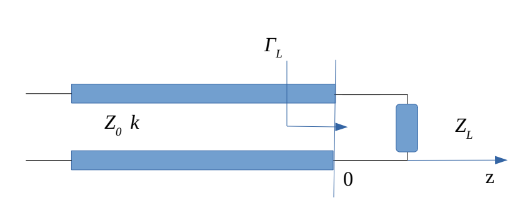
\includegraphics[width=0.8\textwidth]{Images/figure15.png}
\end{center}
Dove avremo i seguenti andamenti di tensione e corrente lungo la linea:
\begin{equation*}
    \begin{dcases}
    V(z) = V^+ e^{-jkz}  V^- e^{jkz} = V^+ e^{-jkz} + V^+ \Gamma(0) e^{jkz} = \\
    \quad= V^+ e^{-jkz} + V^+ |\Gamma(0)| e^{j(kz + \Phi_0)}\\
    I(z) = \frac{V^+}{Z_0} + e^{-jkz} - \frac{V^-}{Z_0} e^{jkz} = \frac{V^+}{Z_0} e^{-jkz} - \frac{V^+}{Z_0} |\Gamma(0)| e^{j(kz + \Phi_0)} 
    \end{dcases}
\end{equation*}

E in generale la potenza vale:
\begin{equation*}
    \begin{aligned}
    P(z) &= \frac{1}{2} V(z) I^*(z) = \frac{1}{2} \left( V^+ e^{-jkz} + V^+ |\Gamma(0)| e^{j(kz + \Phi_0)}\right) \\
    &{\left(\frac{V^+}{Z_0} e^{-jkz} - \frac{V^+}{Z_0} |\Gamma(0)| e^{j(kz + \Phi_0)} \right)}^* =\\
    =& \frac{1}{2} \left( V^+ e^{-jkz} + V^+ |\Gamma(0)| e^{j(kz + \Phi_0)}\right) \\
    &\left(\frac{{V^+}^*}{Z_0} e^{jkz} - \frac{{V^+}^*}{Z_0} |\Gamma(0)| e^{-j(kz + \Phi_0)} \right)=\\
    &= \frac{1}{2} \frac{|V^+|^2}{Z_0} - |\Gamma(0)|^2 \frac{1}{2} \frac{|V^+|^2}{Z_0} + \frac{1}{2} \frac{|V^+|^2}{Z_0}  |\Gamma(0)| e^{j(kz+\Phi_0)} - \\
       &- \frac{1}{2} \frac{|V^+|^2}{Z_0} |\Gamma(0)| e^{-j(kz+\Phi_0)}
    \end{aligned}
\end{equation*}
Quindi:
\begin{equation*}
    P(z) = \frac{1}{2} \frac{|V^+|^2}{Z_0} - |\Gamma(0)|^2 \frac{1}{2} \frac{|V^+|^2}{Z_0} + j \frac{|V^+|^2}{Z_0} |\Gamma(0)| \sin(2kz +\Phi_0)
\end{equation*}
Anche in questo caso la potenza alla sezione z è costituita da una \textbf{Potenza Attiva} indipendente da z:
\begin{equation*}
    \tag{Potenza Attiva}
    Re\{P(z)\} = \frac{1}{2} \frac{|V^+|^2}{Z_0} - |\Gamma(0)|^2 \frac{1}{2} \frac{|V^+|^2}{Z_0}
\end{equation*}
E da una \textbf{Potenza Reattiva}:
\begin{equation*}
    \tag{Potenza Reattiva}
    Im\{P(z)\} = \frac{|V^+|^2}{Z_0} |\Gamma(0)| \sin(2kz + \Phi_0)
\end{equation*}
Che si \textbf{annulla} per $2kz + \Phi_0 = n\pi$, quindi \textbf{non si annulla} per $z=0$ come nel caso di un carico \textbf{puramente resistivo}.\\ \\
Infatti nel caso di un carico con una \textbf{parte reattiva non nulla} ($Z_l = R_l + j X_l$), è associata la \textbf{potenza reattiva}:
\begin{equation*}
    Im\{P(0)\} = \frac{1}{2} |I(0)|^2 X_l = \frac{|V^+|^2}{Z_0} |\Gamma(0)| \sin(\Phi_0) = 2\w (w_m^l - w_e^l)
\end{equation*}
Dove $w_m^l \ e \ w_e^l$ sommo le \textbf{energie pseudo magnetiche e pseudo elettriche immagazzinate nel carico}.

























